\documentclass[fleqn]{anstrans}
%%%%%%%%%%%%%%%%%%%%%%%%%%%%%%%%%%%
\title{Inception Neural Networks for Isotope Identification}
\author{Samuel Dotson, Mark Kamuda, and Kathryn D. Huff}

\institute{
Dept. of Nuclear, Plasma and Radiological Engineering, University of Illinois at Urbana-Champaign \\
sgd2@illinois.edu
}

%%%% packages and definitions (optional)
\usepackage{graphicx} % allows inclusion of graphics
\usepackage{booktabs} % nice rules (thick lines) for tables
\usepackage{microtype} % improves typography for PDF
\usepackage{xspace}
\usepackage{tabularx}
\usepackage{subcaption}
\usepackage{enumitem}
\usepackage{placeins}
\usepackage{amsmath}
\include{acros}
\newcolumntype{c}{>{\hsize=.56\hsize}X}
\newcolumntype{b}{>{\hsize=.7\hsize}X}
\newcolumntype{s}{>{\hsize=.74\hsize}X}
\newcolumntype{f}{>{\hsize=.1\hsize}X}
\newcolumntype{a}{>{\hsize=.45\hsize}X}
\usepackage{titlesec}
\titleformat*{\subsection}{\normalfont}

\begin{document}
%%%%%%%%%%%%%%%%%%%%%%%%%%%%%%%%%%%%%%%%%%%%%%%%%%%%%%%%%%%%%%%%%%%%%%%%%%%%%%%%

\section{Introduction}
The development of algorithms that can accurately identify the isotopic sources of low-resolution gamma-ray 
spectra is an advancement in current spectroscopy workflows \cite{rawool-sullivanStepsAutomatedGamma2010}.
Previous work shows how isotope identification can be performed using 
artificial neural networks 
\cite{kamudaAutomatedIsotopeIdentification2017,kamudaComparisonMachineLearning2018a,kamudaMachineLearningApproach2018}. 
This paper introduces a new feature to the existing architecture of the Artificial Neural Network for Spectroscopic Analysis ($\textit{annsa}$) package, known as an Inception Neural Network (INN). 
An INN implements inception layers that consist of wide convolution layers with several filters, rather than the typical single-filter layer found in simple convolutional neural networks (CNN).
This paper also demonstrates improved methods for simulating spectra to better emulate the background radiation found in real measurements. 
The features of a gamma-ray spectrum vary depending on the full width at half max (FWHM) of the photopeaks. 
Simultaneously applying multiple filters of different sizes allows an INN to capture more features during a single layer than a CNN. 
We hypothesize that an INN will also be robust to changes in background radiation thereby generalizing the $\textit{annsa}$ framework to more scenarios. 
We compare the accuracy of an INN to a simple CNN to determine if the improvement in accuracy warrants the increased computational complexity. 
Finally, new training data will be obtained through simulations with the GADRAS-DRF software \cite{mitchellGADRASIsotopeID2014}.

\section{Theory -- Artificial Neural Networks}

An artificial neural network (ANN) maps values from ${\mathbb{R}}_{N}$ to ${\mathbb{R}}_{K}$ by mimicking biological 
neurons. Examples of an arbitrary neural net and a single neuron are shown in Figures $\ref{fig:dense-nn}$ and $\ref{fig:neuron}$. 

\begin{figure}[ht]
\centering
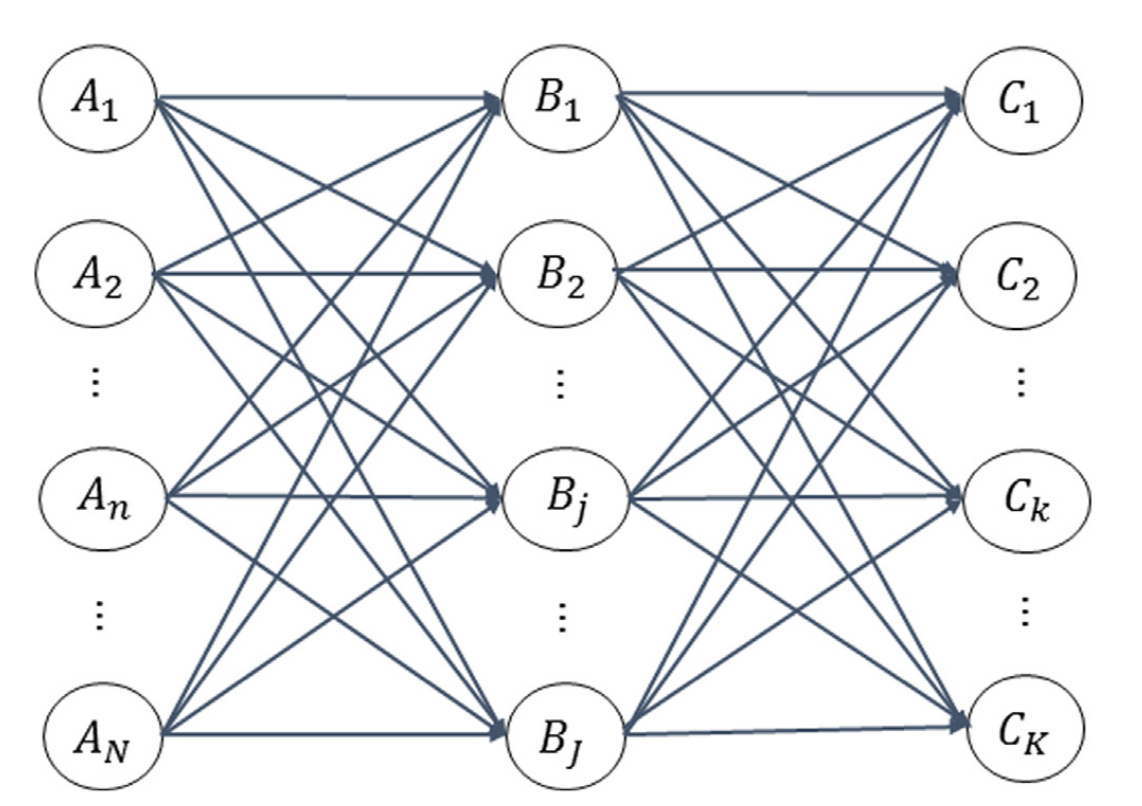
\includegraphics[width=0.5\textwidth]{../figures/dense-layer-figure.png}
\caption{An arbitrary neural network that maps values with weights (arrows) \cite{kamudaComparisonMachineLearning2018a}.}
\label{fig:dense-nn}
\end{figure}
\begin{figure}[ht]
\centering
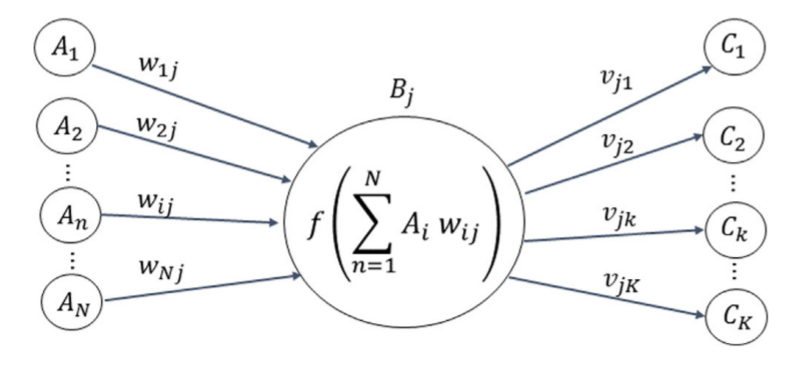
\includegraphics[width=0.5\textwidth]{../figures/neuron-figure.png}
\caption{A single neuron being passed through an activation function, $\textit{f}$ \cite{kamudaComparisonMachineLearning2018a}.}
\label{fig:neuron}
\end{figure}

The sum of the inputs times the weights, $x$, pointing to a neuron are passed through an activation function.
In this paper we used a rectified linear unit ($\textit{relu}$),
\begin{equation}
	\begin{aligned}
		x = \sum_{n=1}^{N}A_i w_{ij} [-],
	\end{aligned}
\end{equation}  

\begin{equation}
	\begin{aligned}
		relu = argmax(0, x) [-],
	\end{aligned}
\end{equation}
The $\textit{relu}$ function will turn $on$ a neuron if $x$ is greater than 0, otherwise the neuron stays off.
The result is used as the input for the next layer, as shown in Figure $\ref{fig:neuron}$ 
An artificial neural network may be trained by iteratively updating the weights of a network by minimizing an error function, $E$. 
The weights are updated through back propagation by taking the derivative of $E$ with respect to the weights. 
The error function minimized during training of the INN is cross-entropy,

\begin{equation}
	\begin{aligned}
		E = -\sum_{c}^{M}y_{o,c}\ln{p_{o,c}} [-].
	\end{aligned}
\end{equation}

Eq. 2 shows the cross-entropy for multiclass classification for cases with more than two possible labels 
for a given input. $M$ is the total number of labels for a given model, in this case it corresponds to 29 
radionuclides \cite{AmericanNationalStandard2016}. Variable $y_{o,c}$ is binary, indicating whether observation, $o$, has the correct label, $c$. 
Variable $p_{o,c}$ is the probability that $o$ is a member of $c$. The complete INN model is shown in Figure $\ref{fig:inn-layer}$ and Figure $\ref{fig:inn-full}$ 
The input for the INN is a 2$"$x2$"$ NaI spectrum of 1024 channels and the final output is a softmax given by,



\begin{equation}
	\begin{aligned}
		softmax(z_j) = \frac{e^{z_j}}{\sum_{k=1}^{k}} [-].
	\end{aligned}
\end{equation}


\begin{figure}[ht]
    \centering
    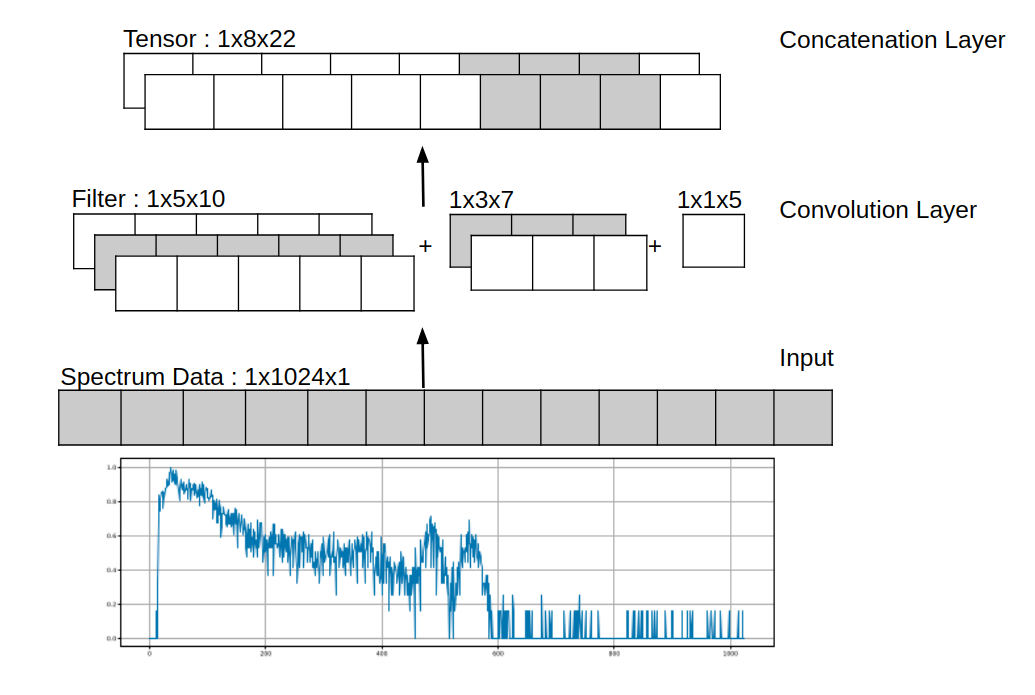
\includegraphics[width=0.5\textwidth]{../figures/inn_layer_improved.png}
    \caption{A gamma spectrum shown as the input for the first inception layer.}
    \label{fig:inn-layer}
\end{figure}
\begin{figure}[ht]
    \centering
    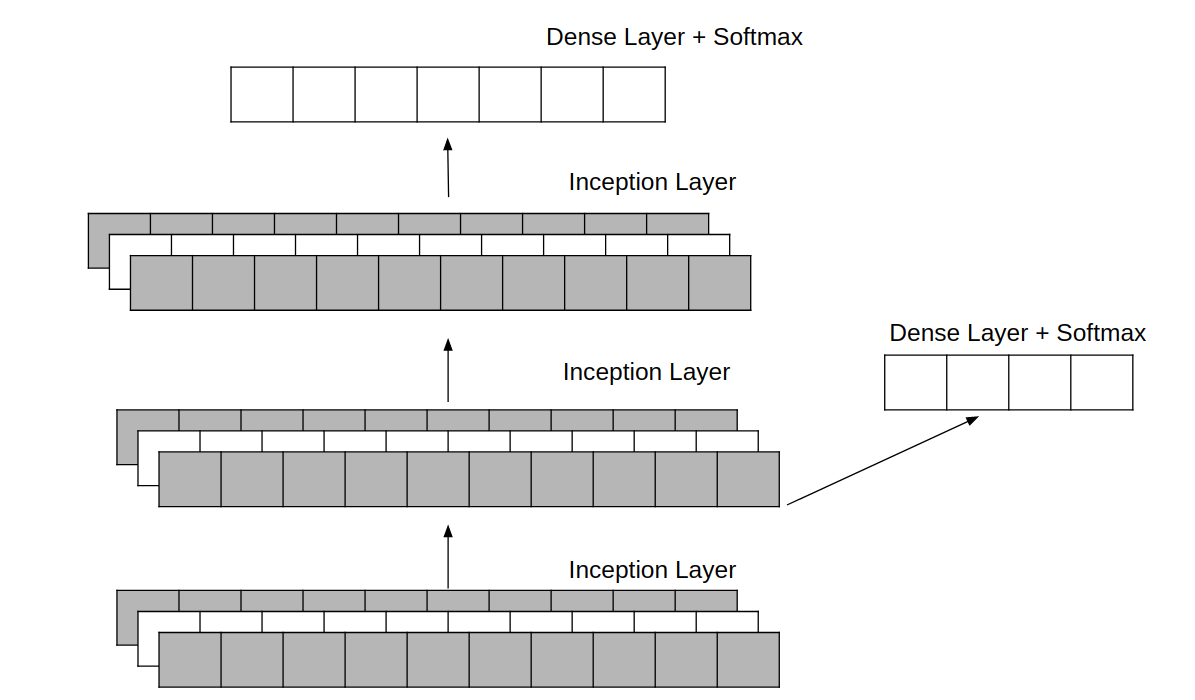
\includegraphics[width=0.5\textwidth]{../figures/inn-full-figure.png}
    \caption{A zoomed out example of a full inception neural network.}
    \label{fig:inn-full}
\end{figure}

The input data is passed through three inception layers and, after flattening, the output is passed to a dense layer which gives the final softmax output. 
Each inception layer typically has a bottleneck, a convolution, and a 
concatenation \cite{szegedyGoingDeeperConvolutions2014,szegedyRethinkingInceptionArchitecture2015}.
The input spectra are a one-dimensional array with length equal to the number of channels in the detector. The purpose of the bottleneck is to reduce dimensionality without losing information. The bottleneck layer is ignored in this research because spectra are already 1D arrays.   
The convolution layer uses filters to select features of a spectrum with local spatial significance and lack long-range relationships. 
Once the convolution has been done with several filters in parallel, the outputs of each of those convolutions are concatenated into a single tensor and passed to the next inception layer, or dense layer if the last layer has been reached. 
Just like a typical CNN, shown in Figure $\ref{fig:cnn}$, the final step after feature identification is classification. 
Classification is performed by using a dense, or fully connected, layer with weights corresponding to a probability for a certain label. 
In this case, the corresponding labels are radionuclides.

\begin{figure}[ht]
	\centering
	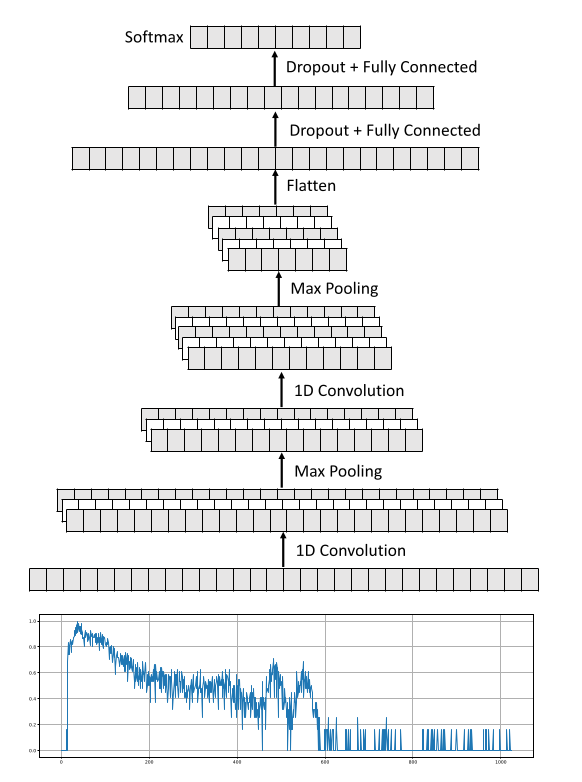
\includegraphics[width=0.5\textwidth]{../figures/cnn-figure.png}
	\caption{An example of a typical convolutional neural network \cite{kamudaComparisonMachineLearning2018a}.}
	\label{fig:cnn}
\end{figure}

\section{Methods}
\subsection{$\textit{Training Set Creation}$}
It is infeasible to obtain enough real gamma spectrum measurements to properly train a neural network. 
Thus all of the datasets used to train the neural network were simulated using GADRAS-DRF \cite{mitchellGADRASIsotopeID2014}. 
The 29 isotopes in the dataset are based on the American National Standards Institute performance criteria for handheld instruments for the detection and identification of radionuclides, ANSI N42-34-2015 \cite{AmericanNationalStandard2016}. 
Previous work \cite{kamudaComparisonMachineLearning2018a} used a uniform distribution of background isotopes and a constant average count of 65 counts per second (cps) for the background. 
Simulating background radiation in this manner fails to capture the variability of real background spectra.
We are updating the simulation protocol to include variations in background conditions. New simulated data will include random noise in a range of 40 to 200 cps. 
We believe this range is realistic for background radiation.

\subsection{$\textit{Network Structure and Hyperparameters}$}
A neural network can memorize training sets resulting in overtraining and a misidentification of novel data. 
This is especially true for an INN, whose weights are difficult to tune with simple back propagation.
To solve this problem during training, we include an intermediate softmax output allowing for error corrections before the entire forward pass is complete. 
This branch is ignored during prediction, but offers a way to prevent overtraining. 
In the fully connected layer, dropout regularization forces the neural network to learn new pathways. 
Hyperparameters can be used to optimize performance and prevent overfitting of the model.
There is no way to know which hyperparameters will influence the model before training, so a random hyperparameter search is performed to find a set of hyperparameters close to the ideal set\cite{bergstraRandomSearchHyperParameter}. 
For CNN structures, like the INN, hyperparameters include the sizes of convolutional filters, the output size (how many filters of each size), the number of nodes in a dense layer, and dropout rate \cite{kamudaMachineLearningApproach2018} shown in Table \ref{tab:hyper}. We also include two INN-specific hyperparameters: Number of inception layers and number of filters per layer. Having a choice in the number of filters exemplifies the benefit of using an INN. Instead of convolving an input with filters of only a single size we can convolve many filter sizes and then concatenate the result as in Figure \ref{fig:inn-layer}.

\begin{table}[ht]
\caption{Hyperparameter Space for INN}
\centering
\begin{tabular}{l r}
\hline\hline
Hyperparameter & {Values}\\
\hline
\#inception layers & {1,2,3}\\
\#filters & {3,4,5}\\
output size & {3,5,7,9,11}\\
kernel size & {5, 10, 15, 20, 25, 30, 35,}\\ 
			& {40, 45, 50, 55, 60}\\
dropout rate & {{0.0, 0.1, 0.2, 0.3, 0.4, 0.5}}\\ 
dense layer size & {32, 64, 128, 256}\\
\hline
\end{tabular}
\label{tab:hyper}
\end{table}

\subsection{$\textit{Benchmark Techniques}$}

In order to compare the efficiency of an INN to a traditional CNN we will use the data and results from \cite{kamudaMachineLearningApproach2018} to train and benchmark the INN. Then we will retrain the CNN and the INN using new and varied data. These comparisons will allow us to determine if, and by how much, an INN is an improvement over a CNN. It will also show us how dataset creation affects the robustness of the models.   
The INN will be considered superior to CNN performance if equivalent training reduces prediction variance. 
For concreteness, a 10$\%$ increase in training time should correspond to a 10$\%$, or greater, decrease in the variance for the INN when compared with the training time and variance of the CNN.

\section{Conclusion}

In this study, we compare the accuracy of two neural networks, a convolutional neural network with two convolutional layers and an inception neural network with three inception layers, for identifying radioactive isotopes in low-resolution gamma-ray spectra. 
We hypothesize that an INN will exhibit an increase in robustness commensurate to its computational complexity and training the neural networks with larger and varied datasets will also improve their robustness. 
Improvements to the identification of isotopes present in a sample of radioactive material will have implications for national security and nuclear nonproliferation.

\section{Acknowledgments}

This work was funded by the Consortium for Verification Technology under Department of Energy National Nuclear Security Administration award number 
DE-NA0002534.  

%%%%%%%%%%%%%%%%%%%%%%%%%%%%%%%%%%%%%%%%%%%%%%%%%%%%%%%%%%%%%%%%%%%%%%%
\bibliographystyle{ans}
\bibliography{bibliography.bib}
\end{document}
